\chapter{Experiments and discussions}
\section{Experimental setup}\label{sec:setup}
% \subsection{Experimental environment}

\subsection{Configurations for market and client models}
For empirical evaluation, we consider the following market with two economy states $\mathcal Y=\{1,2\}$. $1$ is a bad economy and $2$ is a good one. Based on \citeA{chauvet2006dating}, we set the transition matrix for the economy states is given by $$P=\begin{bmatrix}
0.95 & 0.05\\
0.1 & 0.9
\end{bmatrix}$$ indicating that there's a high probability that the economy state stays the same but there's also positive probability to escape. The initial economy is set to be the bad one, i.e. $y_0=1$.

In the bad economy, the risk-free asset has zero return rate, while the risky asset has return drawn from $\mathcal N(0.01,0.05^2)$. In the good economy, the risk-free asset has a return rate of $0.01$ and the risky asset has return drawn from $\mathcal N(0.03, 0.1^2)$. Using the notations introduced in Section \ref{sec:market_model}, we have
    \begin{align*}
    r(y)=\begin{cases}0.00,&y=1\\
    0.01, & y=2
    \end{cases},\qquad
    \mu(y)=\begin{cases}0.01,&y=1\\
    0.03, & y=2
    \end{cases},\qquad
    \sigma(y)=\begin{cases}0.05,&y=1\\
    0.1, & y=2
    \end{cases}.\qquad
    \end{align*}

Unless otherwise specified, we set the time horizon $T$ to be $12$ and the interaction interval to be $3$, indicating a one-year robo-advising product with quarterly interactions.

As for the client, unless otherwise specified, we set the personalized parameters as follows\begin{align*}
    \gamma_0=4,\quad \alpha=0.01,\quad \beta=4,\quad p_\epsilon=0.05,\quad \sigma_\epsilon=0.64.
\end{align*}

Given the configuration for the market, client and the robo-advisor models, we run backwards induction as a one-time pre-processing step to find the optimal strategy at all timestamps given all possible states $\tilde d$. Then, for all the experiments we conduct, we simulate the market and run the robo-advising algorithm for an extensive number of trials and report the mean values for statistical significance.

\subsection{Implementation details}
We implement our robo-advising algorithm in Python\footnote{https://www.python.org/} and SciPy \cite{2020SciPy} and run all experiments on Linux 20.04 LTS in a consumer-level machine equipped with Ryzen 9 5900HS and 32 GB of RAM. Our implementation follows Algorithm \ref{alg2} with approximation as described in Section \ref{sec:approx}. A single run of the backwards induction algorithm to find values at all grid points of $\tilde{\mathcal{D}}_n$ took less than three hours. Although the algorithm has been described in great detail in Section \ref{sec:comp}, we specify the following important implementation details.

\subsubsection{Discretization configuration}
As suggested by Theorem \ref{thm:disc}, for each $n$, we need to evaluate the values of $\mu_n^a,\mu_n^{az},\mu_n^{bz},\mu_n^{bz^2},\tilde\pi_n^*,\allowbreak a_n,b_n$ given all possible states $\tilde d_n\in\tilde{\mathcal D}_n$. Therefore, we discretize the space $\tilde{\mathcal D}_n$:\begin{enumerate}
    \item For economy states at current time and the most recent interaction time, which is discrete, we naturally enumerate all the possible values in $\mathcal Y={1,2}$.
    \item For cumulative excess returns, we consider a range of $[-0.5,0.5]$ and discretize the range with a grid size of $0.1$.
    \item For risk aversion values, we consider a range of $(0,10]$ and discretize the range with a grid size of $0.5$.
\end{enumerate} This is a reasonable discretization grid because in our experiments, as the values almost never fall out of the specified ranges.

In backwards induction, for all $n$, we fill in the values of $\mu_n^a,\mu_n^{az},\mu_n^{bz},\mu_n^{bz^2},\tilde\pi_n^*,\allowbreak a_n,b_n$ at all grid points in $\tilde{\mathcal D}_n$. For querying data at states which are not a grid point, we use linear interpolation \cite{meijering2002chronology} to construct reasonable new data points from values at neighbor grid points. 

\subsubsection{Approximate integration over $\epsilon$}

Note that as pointed in the proof of Theorem \ref{thm:disc}, one need to integrate over the randomness of $\epsilon=\epsilon_{\tau_n+1}+\ldots+\epsilon_{n+1}$ whose distribution is a $\phi$-fold convolution of $\epsilon_n$ whose distribution is defined in Equation \eqref{eq:eps}. Note that this is not trivial to integrate because the probability density function for each $\epsilon_n$ is not continuous, i.e.$$f_{\epsilon_n}(x)=\begin{cases}
    \frac{p_\epsilon}{\sigma_\epsilon}\varphi\left(\frac{x}{\sigma_\epsilon}\right), \qquad &x\neq 0\\
    (1-p_\epsilon)+\frac{p_\epsilon}{\sigma_\epsilon\sqrt{2\pi}}, &x=0
\end{cases}$$ where $\varphi(\cdot)$ is the probability density function for the standard Gaussian $\mathcal N(0,1)$.

We take an approximation approach by first evenly taking many values from the range of $\epsilon_n$ and treat $\epsilon_n$ as a discrete random variable. We calculate the probability mass function for this approximate discrete random variable, and apply Fast Fourier Transform convolution \cite{brigham1988fast} to find the probability mass function for $\epsilon=\epsilon_{\tau_n+1}+\ldots+\epsilon_{n+1}$, and using the PMF to calculate the expectation over the randomness of (now discrete) $\epsilon$. Thus, we transform a difficult integration operation into a weighted sum. To be more specific, we evenly take $65$ points from $[-2,2]$ to form the discrete random variables. We take odd number of points to make sure to include the probability of the outlier point $0$.

\section{Optimal investment strategy}\label{sec:opt}

\begin{figure}[t]
    \centering
    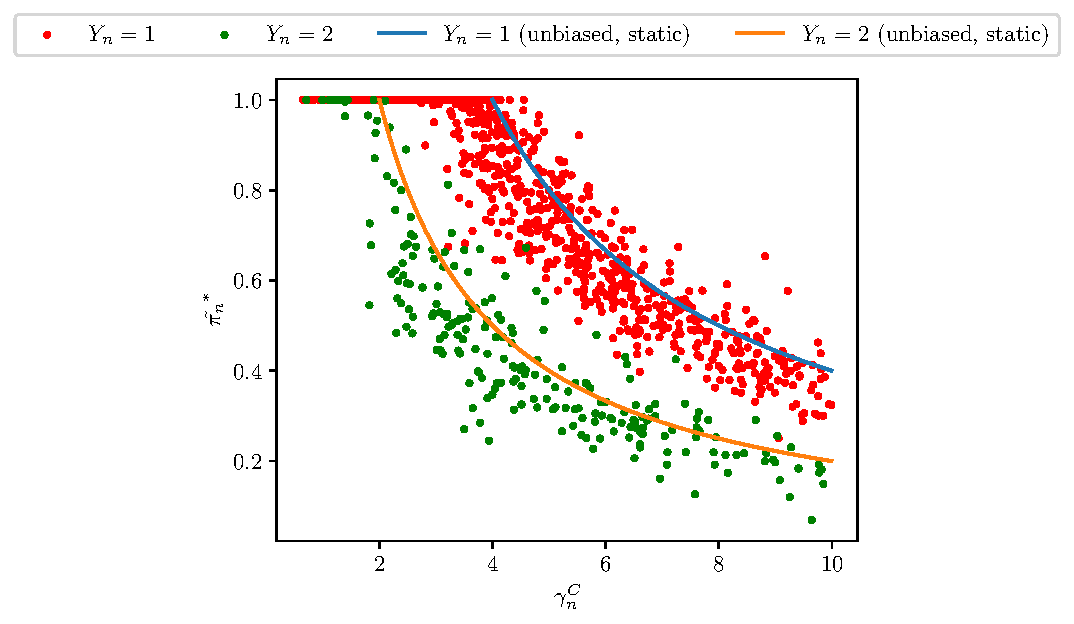
\includegraphics[width=0.9\textwidth]{imgs/optimal_strategy.pdf}
    \caption{Optimal investment strategy as a function of client's risk aversion.}
    \label{fig:opt}
\end{figure}

Experimental configuration follows Section \ref{sec:setup}. We report in Figure \ref{fig:opt} the optimal proportion of wealth allocated to the risky asset, $\tilde\pi_n^d$, as a function of client's risk aversion, $\gamma_n^C$, six months after the start of the investment process, i.e., $n=6$. Each scatter point in the figure represents a trial of market simulation and robo-advisor's response. Green points represents $Y_n=1$, indicating a bad economy at the reported timestamp and red points represents $Y_n=2$, indicating a good one. We also plot (in solid lines) the optimal strategy at $n=6$ as a one-stage mean-variance optimization without behavioral bias, which, as shown in the proof of Theorem \ref{thm:action2gamma}, is given by $$\tilde\pi_n^{C}(\gamma_n^C):=\frac{\mu(Y_n)-r(Y_n)}{\sigma^2(Y_n)\gamma_n^C}.$$ Hence, $\tilde\pi_n^C$ is greater when $Y_n=1$ than $Y_n=2$ (i.e., the solid blue line is above the solid orange line) because $\tilde\pi_n^C=4/\gamma_n^C$ when $Y_n=1$ while $\tilde\pi_n^C=2/\gamma_n^C$ when $Y_n=2$.

First, we note that there are more scatter points with $Y_n=1$ than with $Y_n=2$. This is because the simulation starts at $Y_0=1$ and according to the transition matrix $P$, there's a much higher probability of staying in the same economy state than escaping. Also, we note that even though with same $\gamma_n^C$ and economy state $Y_n$, there are points with different optimal strategies, this is because the optimal strategy $\tilde\pi_n^*$ given by the robo-advisor also depends on the previous market performance and the client's behavioral bias. In each case of $Y_n$, Figure \ref{fig:opt} shows clear trends of $\tilde\pi_n^*$ inversely proportional to $\gamma_n^C$, which agrees with the common sense that higher risk aversion leads to less proportion of wealth allocated to the asset. Figure \ref{fig:opt} also shows that all $\tilde\pi_n^*$ values are concentrate around their respective $\tilde\pi_n^C$ values with the same $Y_n$, which makes sense because the robo-advisor's optimal strategies are approximately behaviourally biased client's optimal strategies. This also verifies the correctness of our implemented algorithm.

At last, for both cases of $Y_n$, we notice that $\tilde\pi_n^*$ is more likely to be smaller than $\tilde \pi_n^C$ rather than larger (for example, most of the red scatter points around the blue solid line are below the line rather than above), indicating that the behavioral bias is more likely to increase client's risk aversion, i.e., $\gamma_n^Z>1$. This is because $$\E[\gamma_n^Z]=\E\left[\exp\left(-\frac{\beta}{\phi}\sum_{k=\tau_n-\phi}^{\tau_n-1}(Z_{k+1}-\mu_{k+1})\right)\right]$$ where each term $Z_{k+1}-\mu_{k+1}$ follows a normal distribution with zero mean and positive variance. Hence, ${\beta}/{\phi}\cdot \sum_{k=\tau_n-\phi}^{\tau_n-1}(Z_{k+1}-\mu_{k+1}))$ follows a normal distribution of zero mean and positive variance, denoted as $\sigma_z^2$. Therefore, we have $\E[\gamma_n^Z]=\exp{(\sigma_z^2/2)}>1$, thus magnifying risk aversion and leading to lower proportion of asset allocated to the risky asset on average.

Figure \ref{fig:opt} is consistent with the findings of \citeA{capponi2022personalized}, but we also include discussions on the effects of economy states by distinguishing $Y_n=1$ and $Y_n=2$ scenarios.

\section{Robo-advisor's personalization measure}\label{sec:personalize}
As shown in Section \ref{sec:opt}, the divergence between the robo-advisor's responding optimal strategy, $\tilde\pi_n^*$, and the client's single-stage greedy optimal strategy with unbiased risk aversion $\gamma_n^C$, $\tilde\pi_n^C$, is caused by the client's behavioral bias. Naturally, one would like to examine the magnitude of such divergence as a measure of the robo-advisor's personalization measure. Since the divergence between $\tilde\pi_n^*$ and $\tilde\pi_n^C$ is originated from the difference in $\gamma_n^C$ and $\gamma_n^R$, \citeA{capponi2022personalized} propose the following personalization measure as a function of interaction interval $\phi$ and behavioral bias parameter $\beta$\begin{equation}
    \mathcal R(\phi,\beta):=\E\left[\frac1T\sum_{n=0}^{T-1}\left|\frac{\gamma_n^C}{\gamma_n^R}-1\right|\right].
\end{equation}

Before experiments, we have a few hypothesis on the properties of $\mathcal R$:\begin{enumerate}
    \item Since the personalization measure $\mathcal{R}$ measures the difference between $\gamma_n^C$ and $\gamma_n^R$, that is, it measures $|\gamma_n^Z|$, the magnitude of the behavioral bias, we expect the lower level of personalization (i.e., higher $\mathcal R$ value) to decrease with an increase in $\beta$, which indicates stronger behavioral bias.
    \item The robo-advisor estimates $\gamma_n^C$ via interactions with the client, hence, we may expect higher level of personalization (i.e., smaller $\mathcal R$ value) with smaller $\phi$ and more frequent interactions. However, interactions are also the reason that gives rise to the existence of behavioral bias, and too frequent interactions will cause a surge in bias $\gamma_n^Z$ and hence results in lower personalization level. 
\end{enumerate}

\begin{figure}[t]
    \centering
    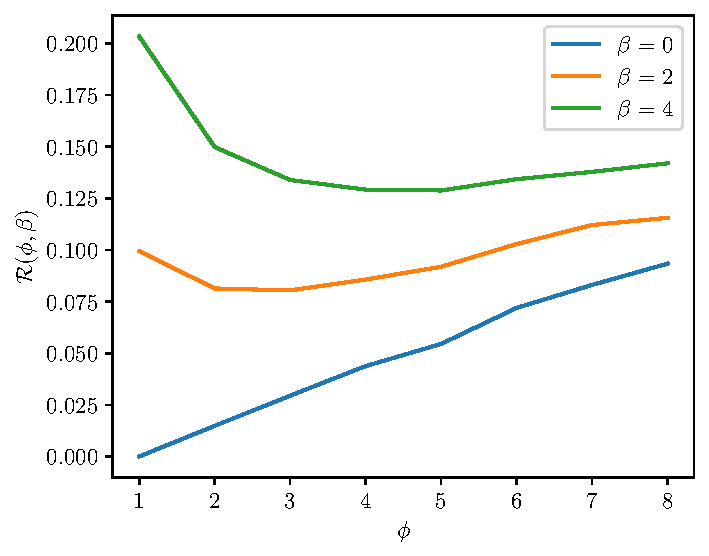
\includegraphics[width=87mm]{imgs/personalization.pdf}
    \caption{Robo-advisor's personalization measure $\mathcal R(\phi,\beta)$ as a function of $\phi$ and $\beta$ on a time horizon of $T=36$.}
    \label{fig:personalization}
\end{figure}

To confirm the hypothesis, we run the robo-advising algorithm and report its personalization measure $\mathcal R(\phi,\beta)$ in Figure \ref{fig:personalization}, with varying $\phi\in\{1,2,3,\ldots,8\}$ and $\beta\in\{0,2,4\}$ values. Note that to better demonstrate the effects of $\phi$, we run for an extended period time with a time horizon of 3 years, i.e., $T=36$. Otherwise, for $T=12$ as in previous experiments, $\phi=6,7,8$ will all lead to only two interactions.

\paragraph{Effects of $\beta$.} As reported in Figure \ref{fig:personalization}, one can clearly note that given the same interaction schedule, robo-advisors with higher $\beta$ values will have higher $\mathcal R$, resulting in weaker personalization. This is because higher $\beta$ values means that the client is more behaviorally biased and hence the $\gamma_n^R$ is more biased away from $\gamma_n^C$. When $\beta=0$, $\gamma_n^Z\equiv0$ and there is no behavioral bias. In this case, the only reason that causes $\gamma_n^R$ to be different from $\gamma_n^C$ is the estimation error of the robo-advisor when modelling the client's risk aversion process. This component is the same regardless of the value of $\beta$, and for larger $\beta$ there will be stronger behavioral bias, hence, personalization measure $\mathcal R$ increases (i.e., weaker personalization) with $\beta$.

\paragraph{Effects of $\phi$.} We discuss the effects of $\phi$ when $\beta=0$ first. In this case, there's no behavioral bias included in $\gamma_n^R$ and at all $n$, the robo-advisor maintains its estimation of $\gamma_n^C$ as $\gamma_n^R$ and gets corrected on interaction times as the communicated risk aversion has no behavioral bias. Therefore, if $\beta=0$ and $\phi=1$, i.e., at all times the robo-advisor estimates $\gamma_n^C$ as $\gamma_n^R$ directly from the client's input of unbiased risk, the personalization measure would be zero and the robo-advisor has achieved perfect personalization. When $\phi$ increases, there are less frequent interactions and the robo-advisor is corrected with client's input of $\gamma_n^C$ less less. Hence, $\mathcal R$ increases as $\phi$ increases when $\beta=0$m as shown in Figure \ref{fig:personalization}. When $\beta>0$, we also need to take behavioral bias into consideration. More frequent interactions will let the robo-advisor to adjust its estimation more often, but since behavioral bias is only applied at interaction times, more frequent interactions will also increase the behavioral bias. Therefore, there's a natural trade-off between better estimation of $\gamma_n^C$ and smaller $\gamma_n^Z$ when the robo-advisor tries to model $\gamma_n^R=\E[\gamma_n^C]\gamma_N^Z$. As shown in Figure \ref{fig:personalization}, for both cases of $\beta=2,4$, we note a decrease in $\mathcal R$ when $\phi$ is small and then an increase in $\mathcal R$ when $\phi$ is larger. The first phase is due to the decrease in behavioral bias caused by less frequent interactions, while the second phase is due to worse estimations of $\gamma_n^R$ when the robo-advisor do not have sufficient interactions to correct itself. Figure \ref{fig:personalization} shows that although our setting does not adopt an explicit penalty for each interaction as in \cite{alsabah2021robo}, there's still an implicit penalty caused of interactions by behavioral bias that only occurs at interaction times. One need to first simulate the robo-advisor algorithm to find out the optimal interaction schedule before allowing it to deploy in the reality. For $\beta$, denote the best interaction interval at $\beta$ is $\phi_beta$, then we have is $\phi_0=1$, $\phi_2=3$ and $\phi_4=5$. 

\section{Estimation of client's personalized parameters}

\begin{figure}[t]
    \centering
    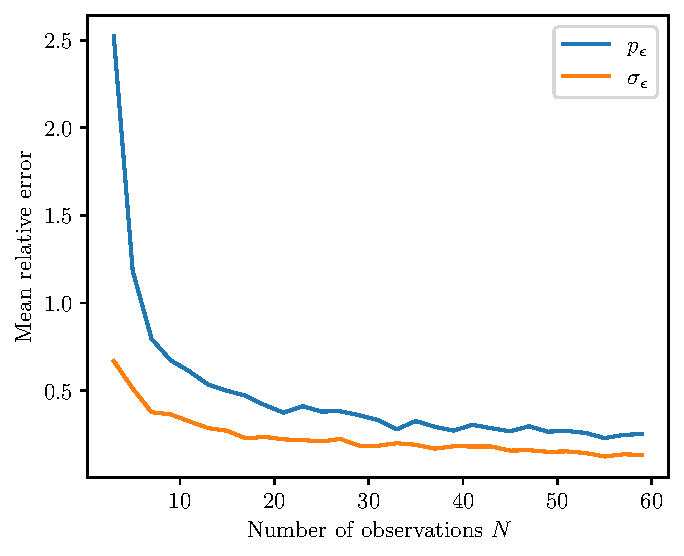
\includegraphics[width=87mm]{imgs/param_estimation.pdf}
    \caption{Mean relative error of estimations of parameters $p_\epsilon$ and $\sigma_\epsilon$.}
    \label{fig:param_estimation}
\end{figure}

At last, we design and conduct experiments to verify the algorithm to estimate the client's personalized parameters as describe in Theorem \ref{thm:est}. In this section, we let the sandbox investment environment to be one with a single economy state and $r=0.05,\sigma=0.2, \mu=0.1$ and fix the ground truth parameters to be $\gamma_0=5,\alpha=0.01,\beta=4,\sigma_\epsilon=1,p_\epsilon=0.5$. We experiment with varying number of observations $N\in[3,61]$. 

As pointed out in Lemma \ref{lem:est_ab}, one can obtain accurate estimations of $\gamma_0,\alpha,\beta$ by setting $N$ to be very small. Hence, we assume the estimator already has the accurate estimations of these variables and focus on the precision of the estimations of $p_\epsilon$ and $\sigma_\epsilon$. We report the mean relative error (MRE) of $p_\epsilon$ and $\sigma_\epsilon$ estimations w.r.t. to number of observations $N$ in Figure \ref{fig:param_estimation}, which is given by \begin{gather*}
    \text{MRE}(p_\epsilon)=\frac1M\sum_{i=1}^{M}\left|\frac{\hat p_\epsilon^{(i)} - p_\epsilon}{p_\epsilon}\right|\\
    \text{MRE}(\sigma_\epsilon)=\frac1M\sum_{i=1}^{M}\left|\frac{\hat \sigma_\epsilon^{(i)} - \sigma_\epsilon}{\sigma_\epsilon}\right|
\end{gather*} where $M=100$ is the number of trials for any $N$ and $\hat p_\epsilon^{(i)}$ is the estimation in the $i$-th trial and $\hat\sigma_\epsilon^{(i)}$ is similarly defined.

It can be seen from Figure \ref{fig:param_estimation} that the MRE of both estimations converges to zero when $N\to\infty$, validating our method of moments for parameter estimation. One can also notice that the MRE of $p_\epsilon$ is consistently higher than $\sigma_\epsilon$. This is because the ground truth value of $p_\epsilon$ is smaller than $\sigma_\epsilon$ and hence a small absolute error in the estimation will lead to a stronger disturbance to the mean relative error. However, Figure \ref{fig:param_estimation} also exposes some limitations of our estimation method. Although our method can give accurate estimations when $N\to\infty$, it takes too many observations to reach usable estimations of the parameters, which is not practical in real-world application. This is also a weakness of method of moments for parameter estimation. Novel and more advanced estimation method can be proposed to address this issue in the future.